%%%%%%%%%%%%%%%%%%%%%%%%%%%%%%%%%%%%%%%%%
% University Assignment Title Page 
% LaTeX Template
% Version 1.0 \left(27/12/12\right)
%
% This template has been downloaded from:
% http://www.LaTeXTemplates.com
%
% Original author:
% WikiBooks \left(http://en.wikibooks.org/wiki/LaTeX/Title_Creation\right)
%
% License:
% CC BY-NC-SA 3.0 \left(http://creativecommons.org/licenses/by-nc-sa/3.0/\right)
% 
% Instructions for using this template:
% This title page is capable of being compiled as is. This is not useful for 
% including it in another document. To do this, you have two options: 
%
% 1\right) Copy/paste everything between \begin{document} and \end{document} 
% starting at \begin{titlepage} and paste this into another LaTeX file where you 
% want your title page.
% OR
% 2\right) Remove everything outside the \begin{titlepage} and \end{titlepage} and 
% move this file to the same directory as the LaTeX file you wish to add it to. 
% Then add \input{./title_page_1.tex} to your LaTeX file where you want your
% title page.
%
%%%%%%%%%%%%%%%%%%%%%%%%%%%%%%%%%%%%%%%%%
%\title{Title page with logo}
%----------------------------------------------------------------------------------------
%	PACKAGES AND OTHER DOCUMENT CONFIGURATIONS
%----------------------------------------------------------------------------------------

\documentclass[12pt]{article}
\usepackage[english]{babel}
\usepackage[utf8x]{inputenc}
\usepackage{amsmath}
\usepackage{graphicx}
\usepackage[colorinlistoftodos]{todonotes}
\usepackage{ dsfont }
\usepackage{amsthm}
\usepackage{ stmaryrd }
\usepackage[]{algorithm2e}
\usepackage{amssymb}
\usepackage{mathrsfs}
\usepackage{float}

\usepackage{caption}
\usepackage{subcaption}

\usepackage{hyperref}
\hypersetup{
    colorlinks,
    citecolor=black,
    filecolor=black,
    linkcolor=black,
    urlcolor=black
}


\newtheorem{definition}{Definition}[section]
\newtheorem{theorem}{Theorem}[section]
\newtheorem{lemma}[theorem]{Lemma}
\newtheorem{proposition}[theorem]{Proposition}
\newtheorem{corollary}[theorem]{Corollary}
\newtheorem*{remark}{Remark}


\begin{document}

\begin{titlepage}

\newcommand{\HRule}{\rule{\linewidth}{0.5mm}} % Defines a new command for the horizontal lines, change thickness here

\center % Center everything on the page
 
%----------------------------------------------------------------------------------------
%	HEADING SECTIONS
%----------------------------------------------------------------------------------------

\textsc{\LARGE University of Nantes}\\[1.5cm] % Name of your university/college
\textsc{\Large Supervised Study Project in Mathematics}\\[0.5cm] % Major heading such as course name

%----------------------------------------------------------------------------------------
%	TITLE SECTION
%----------------------------------------------------------------------------------------

\HRule \\[0.4cm]
{ \huge \bfseries Numerical approximation of the Shallow Water model}\\[0.4cm] % Title of your document
\HRule \\[1.5cm]
 
%----------------------------------------------------------------------------------------
%	AUTHOR SECTION
%----------------------------------------------------------------------------------------

\begin{minipage}{0.4\textwidth}
\begin{flushleft} \large
\emph{Author:}\\
Alexandre \textsc{Mechineau} % Your name
\end{flushleft}
\end{minipage}
~
\begin{minipage}{0.4\textwidth}
\begin{flushright} \large
\emph{Supervisor:} \\

Christophe \textsc{Berthon} % Supervisor's Name
\end{flushright}
\end{minipage}\\[2cm]

% If you don't want a supervisor, uncomment the two lines below and remove the section above
%\Large \emph{Author:}\\
%John \textsc{Smith}\\[3cm] % Your name

%----------------------------------------------------------------------------------------
%	DATE SECTION
%----------------------------------------------------------------------------------------

{\large \today}\\[2cm] % Date, change the \today to a set date if you want to be precise

%----------------------------------------------------------------------------------------
%	LOGO SECTION
%----------------------------------------------------------------------------------------


\includegraphics{logo.png}\\[1cm] % Include a department/university logo - this will require the graphicx package
 
%----------------------------------------------------------------------------------------

\vfill % Fill the rest of the page with whitespace

\end{titlepage}


\begin{abstract}

\addcontentsline{toc}{section}{Abstract}

In this report, the notion of Riemann problem and characteristics will be introduced. With this, we will introduce the Saint Venant equation and numerically study it using finite volumes and Lax-Friedrichs scheme. 
\end{abstract}



\newpage
\tableofcontents

\newpage
\section*{Introduction}
\addcontentsline{toc}{section}{Introduction}
    In this study, we will examine the Saint-Venant equation for shallow water. This equation allows to describe multiple phenomenons like a dam rupture or a tsunami. This equation is obtained from the Naviers-Stokes equation, where horizontal length of the domain is much greater than the vertical height.
    We will start with a theoretical analysis of the transport equation using the characteristics method. We will then extend this method to the nonlinear hyperbolic equation. Using the finite volume method and a Lax-Friedriechs scheme, a solver will be implemented to solve Burger's equation first, then an  equation couple. A source term will, then, be added to obtain the Saint-Venant equation. We will, so, use a well-balanced scheme, described in the reference article, initially of the first order, then of the second order. Finally, we will study the results obtained. We will, mainly, use the results to show that the schemes treat well the discontinuities and  use the last two scheme to study a dam break.


\newpage

\section{Method of characteristics}
    \subsection{Linear advection equation}
        We are going to start from the advection  equation.
        \begin{equation}
            \partial_t\varphi+ a\partial_x\varphi = 0, a \in \mathds{R}
        \end{equation}

        This equation describes the transportation of a quantity by the movement of a quantity at a speed $ a $. To resolve this equation, we can study the \textbf{characteristic curves}, $ X\left(t\right)$:
        \begin{equation}
            \dot X = a, \dot X=\frac{dX}{dt}
        \end{equation}

        Hence, we have :
        \begin{equation*}
            X\left(t\right) = at + x_0
        \end{equation*}

        We can study the solution along the curve $X\left(t\right)$. In this case, we have :
        \begin{equation*}
            \varphi\left(X\left(t\right), t\right) = \Tilde{\varphi}\left(t\right)
        \end{equation*}
        \begin{align*}
            \frac{d\Tilde{\varphi}}{dt} &= \dot X \partial_x\varphi + \partial_t\varphi \\
                                        &= \partial_t\varphi + a\partial_x\varphi\\
                                        &=0
        \end{align*}
        Then, by integration:
        \begin{equation*}
            \Tilde{\varphi} = constant \implies \varphi\left(X\left(t\right), t\right) = \varphi\left(X\left(0\right) , 0\right)
        \end{equation*}
        We add the initial condition, $ \varphi\left(x, t=0\right) = \varphi_0\left(x\right) $.

        We then have, $\varphi\left(X\left(t\right), t\right) = \varphi\left(x_0, t=0\right) = \varphi_0\left(x_0\right)$.

        So we have :
        \begin{equation*}
            \varphi\left(x,t\right) = \varphi_0\left(x- at\right)
        \end{equation*}

        \begin{remark}
            This solution is valid, regardless of the regularity of $\varphi_0$.
        \end{remark}
        
        We can use the previous solution on the following problem:
        \begin{equation*}
            \begin{cases} 
                d_t u + \alpha d_x u = 0\\
                u(x, t=0) = 
                \begin{cases}
                    1 \text{ if } x\in \left[  -1,1\right],\\
                    0 \text{ else}
                \end{cases}
            \end{cases}
        \end{equation*}

        
    
        In this case, the speed of the transportation is $1$. Using the previous result,we can plot the solution:
        
        
        \begin{figure}
            \center
            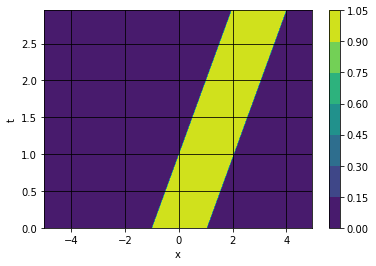
\includegraphics{transport.png}
            \caption{Transport equation with a speed of 1}
        \end{figure}
        

    \subsection{Nonlinear hyperbolic equation}
    
        We can refine the problem and use a non linear function for the flux. We have so: 
        \begin{equation*}
            d_t u+ d_x f\left(u\right) = 0
        \end{equation*}
        More particularly, the inviscid Burgers' equation:
        \begin{equation}
            d_t u + d_x \frac{u^2}{2} = 0, ~f\left(u\right) = \frac{u^2}{2}
        \end{equation}
        If $u$ is {\bf fairly regular} we have :
        \begin{equation*}
            d_x \frac{u^2}{2} = u d_x u
        \end{equation*}
        We can, so, rewrite the inviscid Burgers' equation :
        \begin{equation*}
            d_t u + u d_x u = 0
        \end{equation*}
    
        \begin{remark}
            $d_t u + f^\prime \left(u\right) d_x u = 0$, where $a=f^\prime\left(u\right)$. 
        \end{remark}
    
        We are going to use the same method, previously introduced.
        We define the characteristics curves $X\left(t\right)$ such as:
        \begin{equation*}
            {\dot X}\left(t\right) = f^\prime\left(u \left(X\left(t\right), t\right)\right)
        \end{equation*}
        We are going to study the solution of $u$ along the characteristics curves.
        \begin{equation}
            u\left(X\left(t\right),t\right) = \Tilde{u}\left(t\right)
        \end{equation}
        \begin{align*}
            \frac{d}{d t}\Tilde{u}\left(t\right) &= \dot X d_x u + d_t u \\
                                      &= d_t u + d_x f\left(u\right) = 0
        \end{align*}
        We have, along the characteristics curves, that $u$ is constant.
        \begin{equation}
            u\left(X\left(t\right), u\right) = u\left(X\left(0\right), t=0\right) = u_0\left(x_0\right), ~x_0 = X\left(0\right)
        \end{equation}
        Moreover,
        \begin{align*}
            \dot X\left(t\right) &= f^\prime\left(X\left(u\left(X\left(t\right),t\right)\right)\right) \\
                      &= f^\prime\left(u_0\left(x_0\right)\right) \\
                      &= \text{constant}
        \end{align*}
    
        With that, we can show that:
        \begin{equation}
            X\left(t\right) = f^\prime\left(u_0\left(x_0\right)\right)t + x_0
        \end{equation}
        We search $u_0$ solution of:
        \begin{equation}
            x = f^\prime\left(u_0\left(x_0\right)\right)t + x_0, \text{ where } \left(x,t\right) \text{ are given}
        \end{equation}
        Here, there is two cases defined by the fact if $f$ is an increasing function
        \begin{enumerate}
            \item We assume that $x_0 \mapsto f^\prime\left(u_0\left(x_0\right)\right)$ is increasing.
            
            Hence, the map $x \mapsto f^\prime\left(u_0\left(x_0\right)\right)t + x_0$ is bijective. This imply that the characteristics curves do not cross each other.
            
            \item  We assume that $x_0 \mapsto f^\prime\left(u_0\left(x_0\right)\right)$ is not increasing.
            
            We can then show that, $\exists x_0, x_1 | f^\prime\left(u_0\left(x_0\right)\right) \geq f^\prime\left(u_0\left(x_1\right)\right)$
            We have shown that there is an infinity of solutions. To choose a valid solution, we need to introduce something more.
        \end{enumerate}
        We need to determine the period of time where we can study our problem. We know that we have a problem at the instant where two characteristics curves intersect. Before that, the problem admit a solution using the characteristics curves.
        
        \begin{theorem}
            Let f $\in \mathscr{C}^2, u_0 \in \mathscr{C}^1$ .\\
            Let T =  
            $
            \begin{cases}
                +\infty\text{ if $x_0 \mapsto f^\prime\left(u_0\left(x_0\right)\right)$ is increasing}\\
                - \frac{1}{\min \frac{d}{dx_0}f^\prime\left(u_0\left(x_0\right)\right)}\text{, else}
            \end{cases}
            $
           
            The following Cauchy problem :
            $
            \begin{cases}
                d_t u + d_x f\left(u\right) = 0 \\
                u\left(x,t=0\right) = u_0\left(x\right)
                \end{cases}
            $
            admit a solution $u \in \mathscr{C}^1$ on $[0,T ]$.
        \end{theorem}
        
        We have the solution $u\left(x,t\right)$ where $t\in [ 0, T]$, after the instant $T$ the solution is discontinuous . We are going to use a weak solution to evaluate the solution after the instant $T$.
        \begin{definition}
            We call \textbf{ weak solution} of our problem:
            \begin{equation*}
                 u \in L^\infty_{loc} \left(\mathds{R}\times\mathds{R}^+\right)\text{, such as:}
            \end{equation*}
            \begin{equation*}
                \forall \varphi\in \mathscr{C}^1\left(\mathds{R}\times\mathds{R}^+\right), \int_{\mathds{R}\times\mathds{R}^+} u d_t \varphi + f\left(u\right) d_x\varphi~dx dt = -\int_\mathds{R} u_0\left(x\right) \varphi\left(x, t=0\right)~dx
            \end{equation*}
        \end{definition}   
        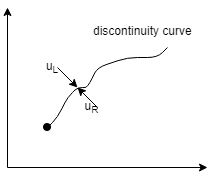
\includegraphics{curve.png}
        
        \begin{lemma}[of Rankine-Hugoniot]
            In a discontinuity, we have :
            \begin{equation*}
                \sigma\left(u_R-u_L\right) + \left(f\left(u_R\right) - f\left(u_L\right)\right)=0
            \end{equation*}
            where $\sigma$ is the propagation speed of the discontinuity.
        \end{lemma}
        
        We can use the previous lemma, we can solve the following problem
        \begin{equation*}
            d_t + d_x\frac{u^2}{2}=0, f\left(u\right)=\frac{u^2}{2}, u_L=2, u_R=0
        \end{equation*}
        Using the lemma of Rankine-Hugoniot, we have:
        \begin{equation*}
            -\sigma\left(0 - 2\right) + \left(\frac{0^2}{2} - \frac{2^2}{2}\right) = 0
        \end{equation*}
        \begin{equation*}
            -\sigma\left(-2\right) + \left(-2\right)=0
        \end{equation*}
        \begin{equation*}
            \sigma=1
        \end{equation*}
        The discontinuity curve is here a line of slope $\sigma$. 
        \begin{remark}
            The discontinuity curves are always lines of slope $\sigma$.
        \end{remark}
    
    \newpage
    
        \subsubsection{Misdefined equation}
            The following problem admit an obvious solution, $u\left(x,t\right) = 0$
            \begin{equation*}
                \left(*\right)
                \begin{cases}
                   d_t + d_x\frac{u^2}{2}=0, f\left(u\right)=\frac{u^2}{2} \\
                   u\left(x,t=0\right)=0
                \end{cases}
            \end{equation*}
            However it's not the only solution, the function $u\left(x,t\right) = 
                \begin{cases}
                    0        &if~x<-\sigma t \\
                    -2\alpha &if~-\sigma t<x<0 \\
                    2\alpha  &if~ 0<x<\sigma t\\
                    0        &if~x>\sigma t
                \end{cases}
                $
            is a weak solution of $\left(*\right)$. In each discontinuity, the lemma of Rankine-Hugoniot is checked.
            We have just shown that we have an infinity of solution, we need to choose the {\bf right} solution. For that, we're going to introduce entropies inequalities.
        
        \subsubsection{Inequalities of entropy}
            We are going to admit that the following problem have a regular solution with uniqueness: 
            \begin{equation}
                \begin{cases}
                    d_t u^\epsilon + d_x f\left(u^\epsilon\right) = \epsilon d_{xx}u^\epsilon \\
                    u^\epsilon\left(x,t=0\right) = u^\epsilon_0\left(x\right)
                \end{cases}
            \end{equation}
            When $\epsilon \to 0^+$, we have $d_t u + d_x f\left(u\right) = 0$ but we loose the uniqueness of the solution. To fix that problem, we are going to introduce a condition that the solution must verify. 
            
            Let $\xi\left(u\right) $ be a convex function of $u$:
            
            \begin{align*}
                \xi^\prime\left(u^\epsilon\right) \left(d_t u^\epsilon + d_x f\left(u^\epsilon\right)\right) &=  \epsilon \xi^\prime\left(u^\epsilon\right)d_{xx}u^\epsilon \\
                d_t \xi\left(u^\epsilon\right) + \xi^\prime\left(u^\epsilon\right)f^\prime\left(u^\epsilon\right)d_x u^\epsilon &= \epsilon \xi^\prime\left(u^\epsilon\right)d_{xx}u^\epsilon \\
            \end{align*}
            We wrote $g= \int \xi^\prime\left(s\right) f^\prime\left(s\right)ds$, then, $\xi^\prime\left(u^\epsilon\right) f^\prime\left(u^\epsilon\right) = g^\prime\left(u^\epsilon\right)$:
            
            \begin{align*}
                d_t\xi\left(u^\epsilon\right) + g^\prime\left(u^\epsilon\right)d_x u^\epsilon &= \epsilon \xi^\prime\left(u^\epsilon\right)d_{xx}u^\epsilon \\
                d_t\xi\left(u^\epsilon\right) + d_x g\left(u^\epsilon\right) &= \epsilon \xi^\prime\left(u^\epsilon\right)d_{xx}u^\epsilon \\
                d_t\xi\left(u^\epsilon\right) + d_x g\left(u^\epsilon\right) &= \underbrace{\epsilon d_{xx}\xi\left(u^\epsilon\right)}_{\substack{ \to 0 \\ \epsilon \to 0}} - \underbrace{\xi^{\prime\prime}\left(u^\epsilon\right)\left(d_xu^\epsilon\right)^2}_{\leq 0}
            \end{align*}
            
            \begin{definition}[Entropic solution]
                A weak solution of $ d_tu+d_xf\left(x\right)=0$ is an {\bf entropic solution} if u verifies the {\bf inequalities of entropy}:
                \begin{equation}
                    d_t\xi\left(u^\epsilon\right) + d_x g\left(u^\epsilon\right) \leq 0, \text{$ \forall g $ convex}
                \end{equation}
            \end{definition}
            
            With that new definition for the weak solution, we have the uniqueness of the solution.

    \subsection{Riemann problem}
        We are going to study a particular Cauchy problem and use the previous inequalities of entropy to determine the solution.
        \begin{equation}
            d_t u + d_x f\left(u\right) = 0,\text{ f a {\bf convex} function}
        \end{equation}
        With the initial condition :
        \begin{equation*}
                u\left(x,t=0\right) = 
                 \begin{cases}
                    u_L & \text{if $x < 0$}\\
                    u_R & \text{if $x \geq 0$}
                \end{cases}  
        \end{equation*}
        We study the solution of the Riemann problem in $\frac{x}{t}$, such as $u\left(x,t\right) = v\left(\frac{x}{t}\right)$.
        There are three solutions possible to the problem which are defined by the initial condition.
        
        \underline{\boldmath \bf If $u_L = u_R$}, implies $ \boxed{u\left(x,t\right) = u_L = u_R}$
        
        \underline{\boldmath \bf If $u_L > u_R$}, the weak entropic solution is a shock (implying that $u$ must check the inequalities of entropies).
        \begin{equation}
                 \boxed{
                u\left(x,t\right) = 
                 \begin{cases}
                    u_L & \text{if $\frac{x}{t} < \sigma $}\\
                    u_R & \text{if $\frac{x}{t} > \sigma $}
                \end{cases}
                }
        \end{equation}
        Where $\sigma$ verifies (Rankine-Hugoniot) :
        \begin{equation*}
            \sigma = \frac{f\left(u_R\right) - f\left(u_L\right)}{u_R - u_L}
        \end{equation*}
        
        \underline{\boldmath \bf If $u_L < u_R$}, in this case, the initial condition is an increasing function. The solution is then a relaxation wave.
        \begin{equation}
                 u\left(x,t\right) = v\left(\frac{x}{t}\right) \implies
                 \begin{cases}
                    d_t u = -\frac{x}{t^2}v^\prime\left(\frac{x}{t}\right) \\
                    d_x u =  \frac{1}{t}v^\prime\left(\frac{x}{t}\right)
                \end{cases}  
        \end{equation}
        \begin{align*}
            d_t u + f^\prime\left(u\right)d_x u &=0 \\
            -\frac{x}{t^2}v^\prime\left(\frac{x}{t}\right) + f^\prime\left(u\right)\frac{1}{t}v^\prime\left(\frac{x}{t}\right) &= 0
        \end{align*}
        Let $\xi= \frac{x}{t}$, we can rewrite the previous equation:
        \begin{align*}
            \frac{1}{t}\left(-\xi + f^\prime\left(u\right)\right)v^\prime\left(\xi\right)&=0 \\
            \frac{1}{t}\left(  -\xi + f^\prime\left(v\left(\xi\right)\right)\right)v^\prime\left(\xi   \right)&=0
        \end{align*}
        
        Hence, we have:
        \begin{equation}
            -\xi + f^\prime\left(v\left(\xi\right)\right) = 0 \text{ or } v^\prime\left(\xi\right)=0
        \end{equation}
        But, we know that $v$ is not constant, so we need to solve:
        \begin{align*}
            -\xi + f^\prime\left(v\left(\xi\right)\right) &= 0 \\
            f^\prime\left(v\left(\xi\right)\right) &= \xi \\
            v\left(\xi\right) &= \left(f^\prime\right)^{-1}\left(\xi\right)
        \end{align*}
        The inverse function, $\left(f^\prime\right)^{-1}$, exists because f is convex.
        Finally, we have, when $u_L < u_R$, 
        \begin{equation*}
             \boxed{
            u(x,t)=
            \begin{cases}
                u_L \text{ if } \frac{x}{t} < f^\prime(u_L)\\
                \left(f^\prime\right)^{-1}\left(x\right) \text{ if } f^\prime(u_L)<\frac{x}{t} <  \frac{x}{t} f^\prime(u_R)\\
                u_R \text{ if } \frac{x}{t} > f^\prime(u_R)
            \end{cases}
            }
        \end{equation*}
\newpage

        For the equation $d_tu+d_x\frac{u^2}{2}=0 $, we obtain the following result, using as initial condition $\begin{cases}u_L = 1\\ u_R =3 \end{cases}$, $\begin{cases}u_L = 3\\ u_R =1 \end{cases}$, respectively. We can easily see the previous result about the relaxation and shock wave.
        
        \begin{figure}[h]
            \centering
            \begin{subfigure}{.5\textwidth}
                \centering
                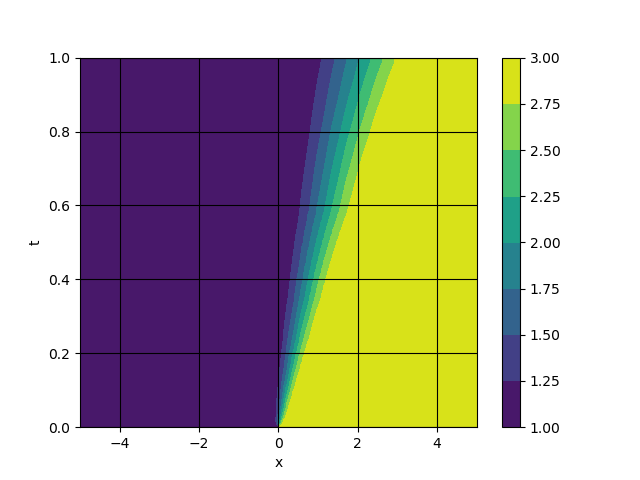
\includegraphics[width=1.1\linewidth]{Burgers13.png}
                \caption{Relaxation wave}
                \label{fig:sub1}
            \end{subfigure}%
            \begin{subfigure}{.5\textwidth}
                \centering
                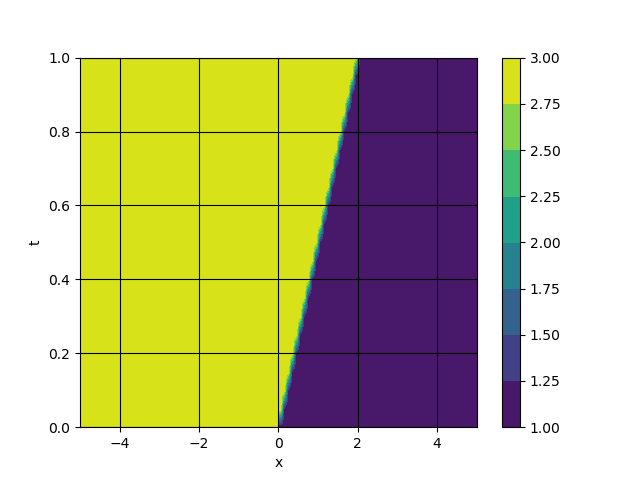
\includegraphics[width=1.1\linewidth]{Burgers31.png}
                \caption{Shock propagation}
                \label{fig:sub2}
            \end{subfigure}
            \caption{Inviscid Burgers' equation}
        \end{figure}
    


\clearpage
\newpage
\section{Saint-Venant, shallow water, equation}
    This equation describe the flow below a free surface(like water/air). The main assumption is that, as the name suggests, the height of the water is smaller than the length of the domain. The equation can be derived from the Naviers-Stokes equation. A second assumption, is that the speed is constant on a column of fluid.
    
    \begin{figure}[H]
        \centering
        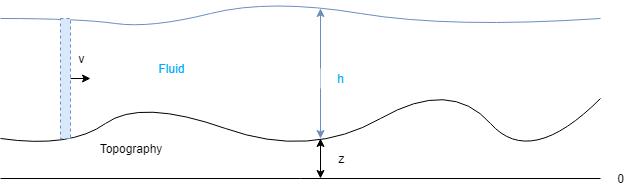
\includegraphics[width=14cm]{modele.png}
        \caption{Context}
        \label{fig:my_domain}
    \end{figure}
    
    \begin{align*}
        &d_t h + d_x(hu) = 0 \\
        &d_t(hu) + d_x\left( hu^2+ \frac{g}{2}gh^2 \right) = - hgz_x
    \end{align*}
    
    The flux of the system is :
    \begin{equation*}
        F(U) = \begin{pmatrix} hu \\ hu^2 + \frac{g}{2}h^2 \end{pmatrix},~where~U=\begin{pmatrix} h \\ hu \end{pmatrix}
    \end{equation*}
    
    
    The main property, which can be useful to check the validity of a scheme, is that a lake at rest keep it state.
    \begin{equation*}
        h + z = Constant, u = 0
    \end{equation*}
            
            
            
            
            
            
            
            
            
            
            
            
            
            
            
    
\newpage
\section{Numerical scheme for  Saint-Venant, shallow-water equation}
    Before solving the Saint-Venant equation numerically, we will start from a simpler model then gradually refine our models to obtain the desired equation. In the first part, we will briefly introduce some details on the discretization , then we will solve the  inviscid Burgers' equation, next we will be solving a coupled equation derived from the  inviscid Burgers' equation. Finally, we will solve, numerically, the Saint-Venant equation.
    
    \subsection{Discretization consideration}
            
        The space domain is divided into $N-1$ intervals, with a constant length $\Delta x$. The function $u$ is approximate using $N$ points.
        The following notation will be used to represent $u$ approximation:
        \begin{equation*}
            u^t_i, \text{ where }
            \begin{cases}
                t\text{: time index}\\
                i\text{: space index}
            \end{cases}
        \end{equation*}
        
        \begin{figure}[h]
            \centering
            \includegraphics[width=15cm]{Discretization.png}
            \caption{Domain discretization}
            \label{discret}
        \end{figure}
        
        
        
        To solve the kind of equation studied, we will be using a finite volume method. This method use the flux given by the equation to compute the quantities incoming and outgoing of given volume called cell. To do that, we will be using a numerical flux, obtained from the Lax–Friedrichs scheme:
        \begin{equation}
            \mathcal{F}(w_L,w_R) = \frac{1}{2}(F(w_L) + F(w_R)) - \frac{\Delta x}{2\Delta t}(w_R-w_L)
        \end{equation}
        
        For the time solving part, we will be using a classic first order finite difference scheme:
        \begin{equation*}
            \frac{du}{dt}\approx \frac{u_i^{t+1}-u_i^t}{\Delta t}
        \end{equation*}
        
            Where $\Delta t$,  will be the best time step given by a  {\bf Courant–Friedrichs–Lewy condition}. The condition will be detailed for each case studied.
            
            
            
            
    
            
        
        
        
        
    
    \newpage
    \subsection{Inviscid Burger's equation}
    
        To begin with, we are going to implement a solver for the following Burger's equation:
        \begin{equation}
            d_t u+d_x F(u)=0, F(u)=\frac{u^2}{2}
        \end{equation}
        
        We have previously obtained result about this class of equation. We will be able to compare the results with the theoretical ones.
        First, we need to compute the numerical flux $\mathcal{F}$, more specifically, the value used. Here, we will be using a simple approximation, the value of $u$ on a volume will be constant:
        
        \begin{figure}[h]
            \centering
            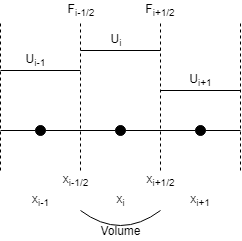
\includegraphics{FluxBurger.png}
        \end{figure}
        
        where 
        \begin{align*}
            \mathcal{F}_{i+\frac{1}{2}}&= \mathcal{F}(u_i, u_{i+1})\\
            \mathcal{F}_{i-\frac{1}{2}}&= \mathcal{F}(u_{i-1}, u_i)
        \end{align*}
        
        The scheme used can be write as:
        \begin{equation}
            u^{t+1}_i=u^t_i - \frac{\Delta t}{\Delta x}(\mathcal{F}_i - \mathcal{F}_{i-1}),i\in\llbracket2,N-1\rrbracket
        \end{equation}
        
        For the boundary condition, we will be using a Dirichlet condition
        \begin{equation*}
             u^{t+1}_i= u_i^0, i \in\{1,N\}
        \end{equation*}
        
        Finally, we need to write the CFL condition. As $f:\mathds{R}\to\mathds{R}$, we have 
        \begin{equation*}
            \frac{\Delta t}{\Delta x}\max_{i\in \llbracket 1,N\rrbracket} |f^\prime\left(x^n_i\right)| \leq \frac{1}{2}
        \end{equation*}
        Hence, we will use the following time step: 
        \begin{equation}
            \Delta t = \frac{\Delta x}{2}\frac{1}{\max_{i\in \llbracket 1,N\rrbracket} |f^\prime\left(x^n_i\right)|}
        \end{equation}
        
        With that in mind, we can write the following algorithm:
        \begin{algorithm}[h]
            \KwData{N : number of points for the space \newline $u_{0_i} = u_0\left(x_i\right)$ \newline T}
            \KwResult{Evaluation of $u\left(x, t=T\right)$ }
            $\Delta x$ = space-step\;
            date = 0.
            $u_0$ contains the values on the current time
            $u_1$ contains the values on the moment computed
            
            \While{date $<$ T}
            {
                 \begin{enumerate}
                     \item Compute dt using the CFL condition
                     \item Compute the flux on each interface
                     \item Compute $u_1(i)=u_0(i) - \frac{\Delta t}{\Delta x}(\mathcal{F}_{i+\frac{1}{2}} - \mathcal{F}_{i-\frac{1}{2}}),~ i\in \llbracket 2,N-1 \rrbracket$
                     \item Apply the boundary condition on $u_1\left(1\right)$ and $u_1\left(N\right)$.
                     \item Swap $ u_0$ and $u_1$
                     \item Increase $date$ by $dt$.
                 \end{enumerate}
            }
        \caption{Lax–Friedrichs method}
        \end{algorithm}
        
    \subsection{Coupled equation}
        We have, now a method to solve numerically the Burger's equation, we are going to use the same method this time, but, with two coupled equations.
        
        \begin{align*}
            d_t h + &d_x hu =0\\
            d_t hu + &d_x (hu^2 + \frac{1}{2}gh^2) =0
        \end{align*}
        
        Where $g$ denotes the gravity.If we set,
        \begin{equation*}
            q= hu \text{, } U = \begin{pmatrix} h\\ q\end{pmatrix}\text{ and } F(U) = \begin{pmatrix} q\\ \frac{q^2}{h} + \frac{1}{2}gh^2\end{pmatrix}
        \end{equation*}
        we have:
        \begin{equation*}
            d_t U+d_x F(U) = 0
        \end{equation*}
        
        Although, we already solved this kind of equation. We just need to detail the computation of u and the CFL condition.
        \begin{remark}
            When we need $u$, the speed, we will use the following:
            \begin{equation*}
                u = 
                \begin{cases}
                    0, h\leq 0\\
                    \frac{q}{h}, h>0
                \end{cases}
            \end{equation*}
        \end{remark}
        The case $ u=0$ if $h\leq 0$ describe the fact that, when there is no fluid, the speed of the fluid is nil.
        
        
        
        We use the same method that for the Burger's equation, so the algorithm is the same.
    
    \newpage
    \subsection{Saint-Venant equation}
        
        We almost have the Saint-Venant equation for shallow water. We just need to take into account the height of the ground. We have so:
        \begin{align*}
            d_t h + &d_x hu =0\\
            d_t hu + &d_x (hu^2 + \frac{1}{2}gh^2) = -hgz_x
        \end{align*}
        
        Like previously, we can rewrite the system using the same notation:
        
        \begin{equation*}
            d_t U+d_x F(U) = \begin{pmatrix}0\\ -hgz_x\end{pmatrix}
        \end{equation*}
        
        We are going to use a well balanced scheme . First, we will be using a first order well-balanced scheme. Then, a second order extension will be implemented.
        
        For the two method, the CFL condition is the same. To compute it, we need the speed of the waves, who is given by the eigenvalues of the jacobian of $F$.
        \begin{equation*}
            q= hu \text{, } U = \begin{pmatrix} h\\ q\end{pmatrix}\text{ and } F(U) = \begin{pmatrix} q\\ \frac{q^2}{h} + \frac{1}{2}gh^2\end{pmatrix}
        \end{equation*}
        \begin{equation*}
            \nabla_U F(U) = \begin{pmatrix} 0& 1 \\ -\frac{q^2}{h^2}+gh &\frac{2q}{h}\end{pmatrix}
        \end{equation*}
        We compute the eigenvalues of $\nabla_U F(U)$
        \begin{align*}
            P(\lambda)  &= | \nabla_U F(U) - I\lambda| = 0\\
                        &= -\lambda (\frac{2q}{h} -\lambda) - (-\frac{q^2}{h^2} + gh)=0\\
                        &= -\lambda (2u-\lambda) + u^2 -h =0\\
                        &= (\lambda -u)^2-gh = 0 \\
                        \implies \lambda^\pm = u\pm \sqrt{gh}
        \end{align*}
        The CFL condition is therefore:
        \begin{align*}
            \frac{\Delta t}{\Delta x}\max_{i\in \mathds{Z}} \left| \lambda ^\pm(U^t_i)\right| \leq \frac{1}{2}\\
            \implies \Delta t= \frac{\Delta x}{2\max_{i\in \mathds{Z}} \left| \lambda ^\pm(U^t_i)\right|}
        \end{align*}
        The index of the quantities used will follow the following diagram:
        \begin{figure}[h]
            \centering
            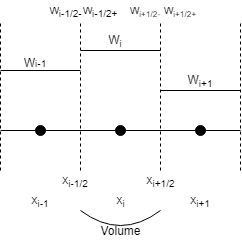
\includegraphics{1storder.png}
            \label{repidx}
        \end{figure}
        
        \subsubsection{Well-balanced scheme: first order}
        But, we are going to use a scheme with a local hydrostatic reconstruction. All quantities are recalculated at the interfaces, using the following formula:
        
        \begin{align*}
            &z_{i+\frac{1}{2}}=\max(z_i, z_{i+1}) \\
            &h_{i+\frac{1}{2}-} = \max(0, h_i+z_i - z_{i+\frac{1}{2}}) \\
            &h_{i+\frac{1}{2}+} = \max(0, h_{i+1}+z_{i+1} -z_{i+\frac{1}{2}}) 
        \end{align*}

        With this new quantities, we can evaluate $U$ around the interface:
        \begin{equation*}
            U_{i+\frac{1}{2}-} =\begin{pmatrix} h_{i+\frac{1}{2}-} \\ h_{i+\frac{1}{2}-}u_i\end{pmatrix} ,U_{i+\frac{1}{2}+} =\begin{pmatrix} h_{i+\frac{1}{2}+} \\ h_{i+\frac{1}{2}-}u_{i+1}\end{pmatrix}
        \end{equation*}
        
        The $+$ and $-$ use in the interface value describe the value taken at the right and the left, respectively, by the interface.
        We have the following relation for a quantities W:
        \begin{align*}
            W_{i-\frac{1}{2}-}=W_{(i-1)+\frac{1}{2}-} \\
            W_{i-\frac{1}{2}+}=W_{(i-1)+\frac{1}{2}+}
        \end{align*}
        The numerical flux is defined with the new value:
        \begin{equation*}
            \mathcal{F}_{i+\frac{1}{2}}= \mathcal{F}(U_{i+\frac{1}{2}-},U_{i+\frac{1}{2}+})
        \end{equation*}
        
        Finally, we write the source term as:
        \begin{equation*}
            S_i = \begin{pmatrix} 0 \\ \frac{g}{2}\left(  h^2_{i+\frac{1}{2}-} - h^2_{i-\frac{1}{2}+} \right)\end{pmatrix}
        \end{equation*}
        
        we then have the following scheme:
        \begin{equation}
            U_i^{t+1} = U_i^t - \frac{\Delta t}{\Delta x}(\mathcal{F}_{i+\frac{1}{2}} - \mathcal{F}_{i-\frac{1}{2}} - S_i),i\in\llbracket2,N-1\rrbracket
        \end{equation}
        
        For the boundary condition, we will be using a Dirichlet condition:
        \begin{equation}
             u^{t+1}_i= u_i^0, i \in\{1,N\}
        \end{equation}
        
        The algorithm used is the same that previously, but, with the source term taken into accout.
        
        \begin{algorithm}[h]
            \KwData{N : number of points for the space \newline $u_{0_i} = u_0\left(x_i\right)$ \newline T}
            \KwResult{Evaluation of $u\left(x, t=T\right)$ }
            $\Delta x$ = space-step\;
            date = 0.
            $u_0$ contains the values on the current time
            $u_1$ contains the values on the moment computed
            
            \While{date $<$ T}
            {
                 \begin{enumerate}
                     \item Compute dt using the CFL condition
                     \item Compute the flux on each interface
                     \item Compute $u_1(i)=u_0(i) - \frac{\Delta t}{\Delta x}(\mathcal{F}_{i+\frac{1}{2}} - \mathcal{F}_{i-\frac{1}{2} }-S_i),~ i\in \llbracket 2,N-1 \rrbracket$
                     \item Apply the boundary condition on $u_1\left(1\right)$ and $u_1\left(N\right)$.
                     \item Swap $ u_0$ and $u_1$
                     \item Increase $date$ by $dt$.
                 \end{enumerate}
            }
        \caption{Well balanced scheme algorithm (First order)}
        \end{algorithm}




        \subsubsection{Well-balanced scheme: second order}
        
        To increase the order of the scheme, we are going to compute a value for each side of a cell ($W_{i,l},~W_{i,r}$). A cell-centered source term, $S_{ci}$, is added to preserve the consistency.
        \begin{figure}[h]
            \centering
            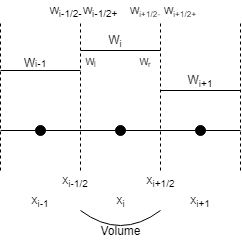
\includegraphics{2ndorder.png}
            \label{2ndorder}
        \end{figure}
        With the following formula for $W_{i,l},~W_{i,r}$:
        \begin{align*}
            &W_{i,l}=w^t_i - \frac{1}{2}\delta w^t_i \\
            &W_{i,r}=w^t_i + \frac{1}{2}\delta w^t_i \\
            &\delta w^t_i = minmod(W_{i} - W_{i-1}, W_{i+1} -W_{i}) \\
            &minmod(x,y) = \begin{cases}  \min(x,y), \text{ if } x,y \geq 0 \\
                                        \max(x,y), \text{ if } x,y \leq 0\\
                                        0, \text{ elsewhere}
                                        \end{cases}
        \end{align*}
        
        The quantities used become:
        \begin{align*}
            &z_{i+\frac{1}{2}} = \max(z_{i,r}, z_{i+1,l})\\
            &h_{i+\frac{1}{2}-} = \max(0, h_{i,r}+z_{i,r} - z_{i+\frac{1}{2}}) \\
            &h_{i+\frac{1}{2}+} = \max(0, h_{i+1,l}+z_{i+1,l} -z_{i+\frac{1}{2}}) \\
            &U_{i+\frac{1}{2}-} =\begin{pmatrix} h_{i+\frac{1}{2}-} \\ h_{i+\frac{1}{2}-}u_{i,r}\end{pmatrix} ,U_{i+\frac{1}{2}+} =\begin{pmatrix} h_{i+\frac{1}{2}+} \\ h_{i+\frac{1}{2}-}u_{i+1,l}\end{pmatrix}
        \end{align*}
        
        The source terms are, then, written as:
        \begin{align*}
            &S_i = \begin{pmatrix} 0 \\ \frac{g}{2} \left(  h^2_{i+\frac{1}{2}-} - h^2_{i,r} + h^2_{i,l} + h^2_{i-\frac{1}{2}+} \right)\end{pmatrix} \\
            &S_{ci} = \begin{pmatrix}  0 \\ g\frac{h_{i,l} + h_{i,r}}{2}(z_{i,l} - z_{i,r})  \end{pmatrix}
        \end{align*}
        
        The second-order well-balanced scheme is, then, written such as:
        
        \begin{equation}
            U_i^{t+1} = U_i^t - \frac{\Delta t}{\Delta x}(\mathcal{F}_{i+\frac{1}{2}} - \mathcal{F}_{i-\frac{1}{2}} - S_i - S_{ci}),i\in\llbracket2,N-1\rrbracket
        \end{equation}
         For the boundary condition, we will be using a Dirichlet condition:
        \begin{equation*}
             u^{t+1}_i= u_i^0, i \in\{1,2,N-1,N\}
        \end{equation*}
        
        The algorithm used is the same as the first order scheme, except the cell-centered source term added.

         \begin{algorithm}[h]
            \KwData{N : number of points for the space \newline $u_{0_i} = u_0\left(x_i\right)$ \newline T}
            \KwResult{Evaluation of $u\left(x, t=T\right)$ }
            $\Delta x$ = space-step\;
            date = 0.
            $u_0$ contains the values on the current time
            $u_1$ contains the values on the moment computed
            
            \While{date $<$ T}
            {
                 \begin{enumerate}
                     \item Compute dt using the CFL condition
                     \item Compute the flux on each interface
                     \item Compute $u_1(i)=u_0(i) - \frac{\Delta t}{\Delta x}(\mathcal{F}_{i+\frac{1}{2}} - \mathcal{F}_{i-\frac{1}{2} }-S_i - S_{ci}),~ i\in \llbracket 3,N-2 \rrbracket$
                     \item Apply the boundary condition on $u_1\left(1\right)$ and $u_1\left(N\right)$.
                     \item Swap $ u_0$ and $u_1$
                     \item Increase $date$ by $dt$.
                 \end{enumerate}
            }
        \caption{Well balanced scheme algorithm (second order)}
        \end{algorithm}

\clearpage
\newpage

\section{Numerical result}
    All previously introduced schemes have been coded in C++. The source code is accessible on \href{https://github.com/Alexsaphir/TER}{Github}. The data obtained were displayed using Paraview or Python.
    
    \subsection{Burger's Equation}
        With this equation, we want to see if the scheme, used is able to verify the analytical properties that we have shown in the first part. To do that, we are going to test the three cases that we have found.
        The initial function is the following:
        \begin{equation*}
            u_0(x) = \begin{cases} u_L , x<0 \\ u_R, x>0  \end{cases}, x\in [-\frac{L}{2},\frac{L}{2}]
        \end{equation*}
        
        Where $L$ is the horizontal length of the domain studied and $u_L,u_R\in \mathds{R}$.
        \begin{itemize}
            \item Let's $u_L=u_R$, the solution is thus $u=u_L=u_R$.
                \begin{figure}[H]
                    \centering
                    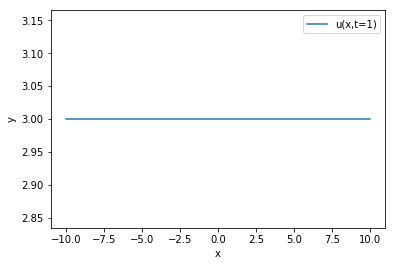
\includegraphics[width= 8cm]{Burgers/Burgers331.png}
                    \label{fig:my_label33}
                \end{figure}
                We can see that the solution is exact.
            \item Let's $u_L=1, u_R = 3$, the solution is a relaxation wave.
                \begin{figure}[H]
                    \centering
                    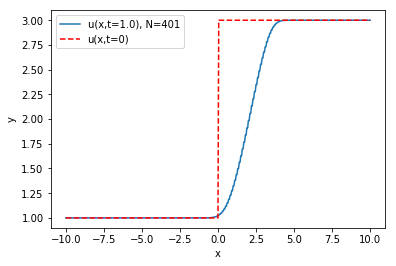
\includegraphics[width= 8cm]{Burgers/Burgers13.png}
                    \label{fig:my_label13}
                \end{figure}
                
            \item Let's $u_L=3,u_R=1$, the solution is a shock wave.
                \begin{figure}[H]
                    \centering
                    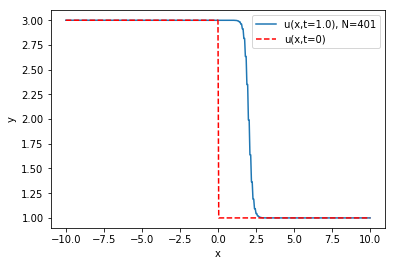
\includegraphics[width= 8cm]{Burgers/Burgers31.png}
                    \label{fig:my_label31}
                \end{figure}
                We can easily see a little bit of dissipation on the shock.
        \end{itemize}
        
        \newpage
        \subsection{Coupled equations}
            We are going to check in a first time that if the initial condition is constant and there is no speed, a lake at rest keep it's current state.
            \begin{figure}[H]
                \centering
                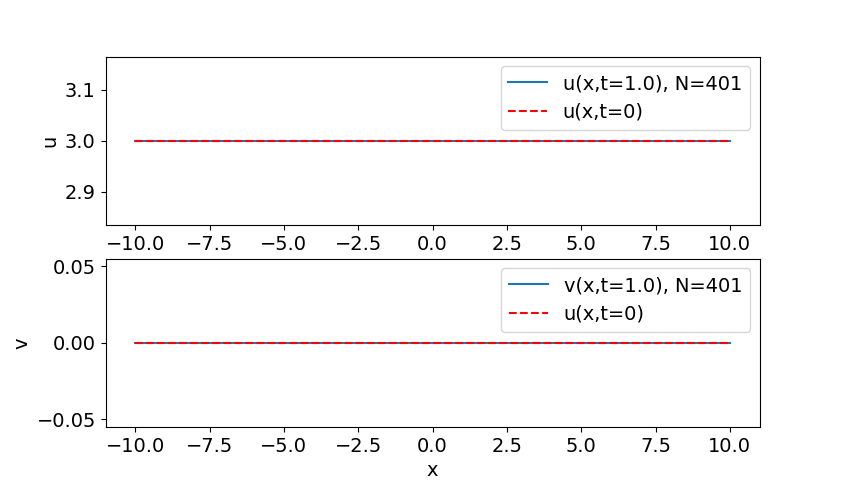
\includegraphics[width= 8cm]{Coupled/Lcst.png}
                \caption{Lake at rest}
                \label{fig:my_CLcst}
            \end{figure}
            
            
            The equation allows to describe a dam break. We are going to use the following condition, with a speed of 0 at the beginning and simulate a dam break. The initial conditions are very rough, we use the same that for a Riemann problem.
            \begin{figure}[H]
                \centering
                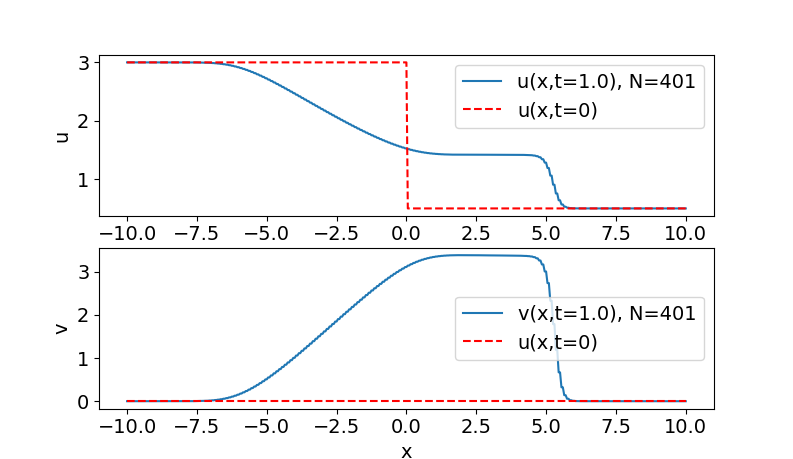
\includegraphics[width= 8cm]{Coupled/Ldam.png}
                \caption{Dam break}
                \label{fig:my_CLdam}
            \end{figure}
        
        
            We can see the relaxation wave and the shock wave easily. The speed also has a particular profile. We see that, during the relaxation period, the speed increases regularly. When the height of water becomes constant, the speed too. During the shock,  there is also a shock in the speed. 
        
        \subsection{Saint-Venant, shallow water, equation}
            The first thing that we can test for each scheme (1st and 2nd order) is that a lake at rest keeps its current state.
            
            \begin{figure}[H]
                \centering
                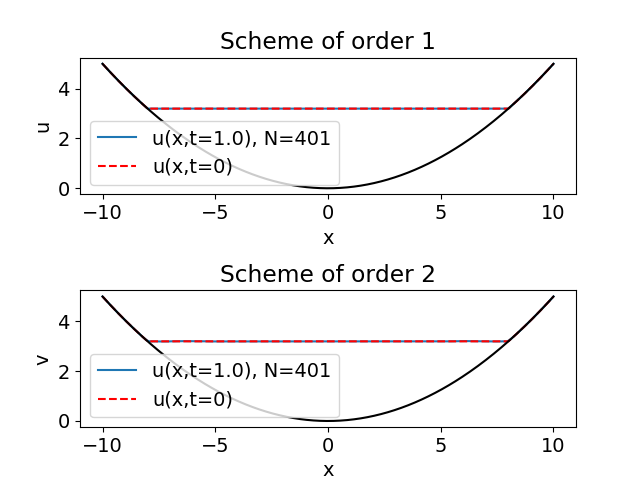
\includegraphics[width= 8cm]{LFSV/L2cst.png}
                \caption{Lake at rest}
                \label{fig:Lcst}
            \end{figure}
            
            We can easily see that both schemes preserve correctly the steady stat of a lake at rest.
            Next, we can simulate a dam break, but this time, with a more real topography.
            \begin{figure}[H]
                \centering
                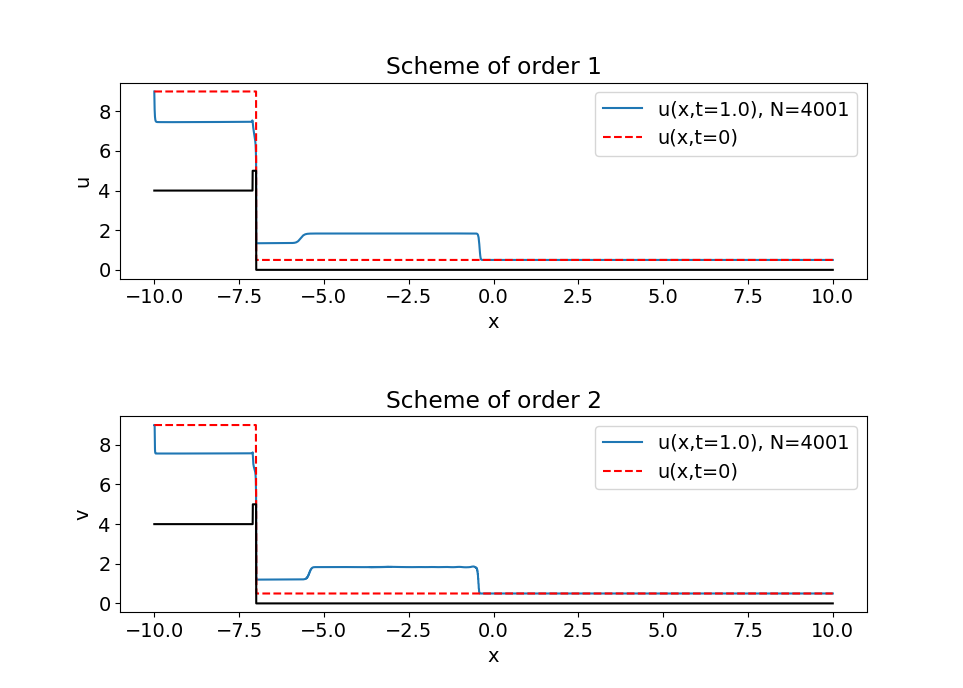
\includegraphics[width= 8cm]{LFSV/dambreakHR.png}
                \caption{Dam break}
                \label{fig:my_db}
            \end{figure}
            We can see that there is a shock wave on the front of the fluid.
            
           
            
            Finally, we are going to simulate an oscillating lake, to compare the performance of each scheme. We use the following condition:
            \begin{align*}
                &z(x) = \frac{1}{2}\left( 1 - \cos{\pi\frac{x-.5}{.5}+1}  \right)\\
                &h(x,t=0) = \max(0, .4 - z(x) + .04\sin{\frac{x - .5}{.25}} - max(0, -.4 + z(x)))
            \end{align*}
            \begin{figure}[H]
                    \centering
                    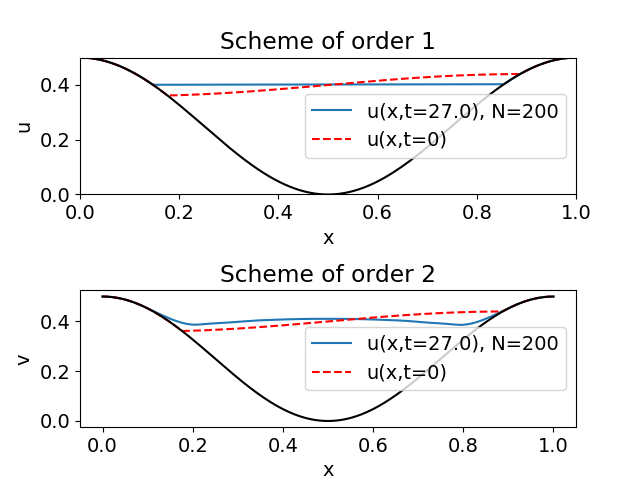
\includegraphics[width= 12cm]{LFSV/L2lake.png}
                    \caption{Oscillating lake}
                    \label{fig:asci}
                \end{figure}
            
            We can see that the perturbations disappear with the first-order scheme. Unlike the second-order scheme, the disturbance is retained.
            
        \newpage
        
        \section{Conclusion}
            
            In this study, we have been able to study a complex coupled equation using mainly the Flux of the equations. We have implemented a solver were the discontinuity was very well taking into account. 
            
            A two dimensional case would allow to use the shallow water equation in some practical case, like a dam break that we have only see in one dimension. We could then study the impact of the rupture of an existing or future dam on a territory. The study of the speed of the wave could allow to know the forces applied by the water.
            
            We could try to improve the result of the well-balanced scheme by using a second order finite difference for the time or by using a non linear grid, where the mesh would be optimized with the value of the function $U$. That is to say, that if U is slowly varying locally  we could use a spatial step greater than where $U$ is varying quickly. The computation of the flux could be improved using an alternative to the Lax-Friedrichs scheme used, like a kinetic solver proposed in the given article. 
            As stated above, an extension to a two dimensional case for the first order scheme could also be realized.

\newpage
\nocite{*}
\bibliographystyle{plain}
\bibliography{main}{}





        
\end{document}